\chapter{Document ranking}
We consider document as binary vector $X, Y \in \{0, 1\}^D$ and we start to use 
as score the \emph{overlap measure} defined as 
\[ |X \cap Y| \]
and in figure \ref{img:overlap} is possible to note that it provides a measure without information.

\begin{figure}
	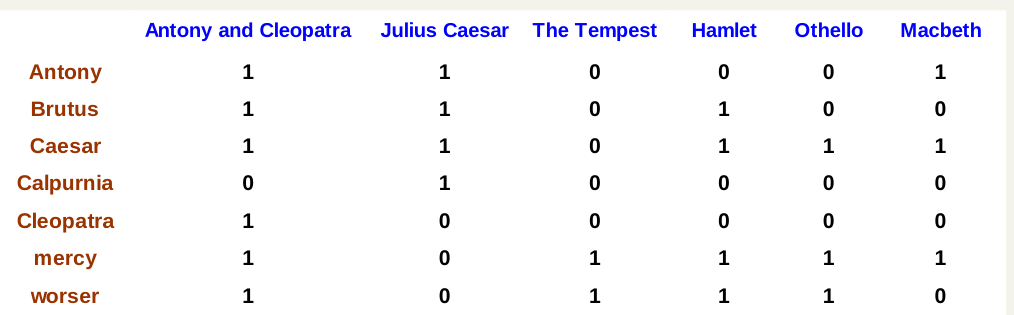
\includegraphics[width=0.8\textwidth]{Images/exampleOverlap}
	\caption{Example of Overlap measure}
	\label{img:overlap}
\end{figure}
Better measures are the following:
\begin{description}
	\item [Dice coefficient: ] with respect to average of $\#$ terms, is not respect triangular rules and it is defined as 
		\[ 2 |X \cap Y| / (|X| + |Y|) \]
	\item [Jaccard coefficient: ] with respect to possible terms, it respects the triangular rules, and it is defined as 
		\[ |X \cap Y| / |X \cup Y| \]
\end{description}
Overlap matching doesn’t consider term \emph{frequency} in a document, term \emph{scarsity} in collection and length of documents so 
score should be normalized, and to do that we introduce now a famous weight \emph{tf-idf}, defined as
\[ w_{t, d} = tf_{t, d} \log \frac{n}{n_t} \]
where we have $tf_{t, d}$ defined as number of occurences of term $t$ in document $d$ and $idf_t = \log (n/n_t)$, 
where $n$ is the number of documents and $n_t$ is the number of docs containing term $t$.

We have also that the distance is a bad idea, as it is possible to note in figure \ref{img:exDistance}, and we define
now the \emph{cosine} measures as follows
\begin{figure}
	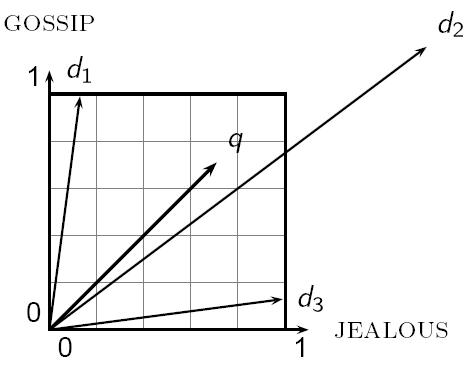
\includegraphics[width=0.7\textwidth]{Images/distanceProblem}
	\caption{Example of problem in distance}
	\label{img:exDistance}
\end{figure}
\[ \cos \alpha = \frac{v * w}{\norm{v} * \norm{w}} \]
The problem is this approach is that it is easy to spam and also that it is computationally infeasible,
cause we have to compute the dot-product $v * w$.

We define also \emph{cosing} measure between query and document in the following way
\[ \cos(q, d) = \frac{q * d}{\norm{q} \norm{d}} = \frac{\sum _{i=1}^{|D|} q_i * d_i}{\sqrt{\sum_{i=1}^{|D|} q_i^2} * \sqrt{\sum _{i=1}^{|D|} d_i^2}} \]
where $q_i$ is the tf-idf weight of term $i$ in the query and $d_i$ is the tf-idf weight of term $i$ in the document.

To help to compute the cosine between query and document we use inverted lists and also that
\[ w_{t, d} = tf_{t, d} \log (n / n_t) \]
that can be computed simultaneously since for every term $t$, we have in memory the length $n_t$ of its posting list and for 
every docID $d$ in the posting list of term $t$, we store its frequency $tf_{t, d}$ which is typically small and 
thus stored with unary/gamma.

In figure \ref{img:computeCosine} it possible to note the algorithm to compute the cosine score and also that 
vector space is okay for bag-of-words queries, that provides clean metaphor for similar-document queries and 
it is not a good combination with operators: boolean, wild-card, positional, proximity.

It was used in first generation of search engines, invented before "spamming" web search, since 
inject webpage with spamming elements that will confuse search engines.

\begin{figure}
	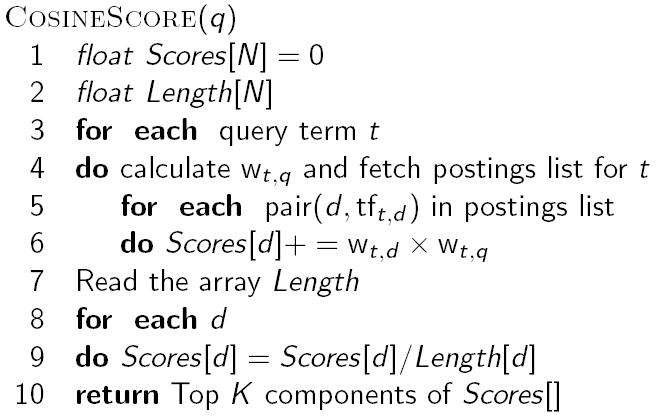
\includegraphics[width=0.8\textwidth]{Images/computeCosineScore}
	\caption{Algorithm to compute the cosine score}
	\label{img:computeCosine}
\end{figure}

\section{Top-k documents}
The computation of $\cos$ is very costly, so to compute the top$-k$ 
documents we find a set $A$ of contenders, with $k < |A| << N$,
where set $A$ does not necessarily contain all top$-k$, but has many
documents from among the top$-k$ and return the top$-k$ docs in $A$,
according to the score; the same approach is also used for other 
scoring functions and we will look at several schemes following this approach.

To select the $A$ docs we consider docs containing at least one query term
and we use the following approaches:
\begin{itemize}
    \item for multi-term queries, compute score for docs containing
	  most query terms (say at least $q-1$ out of $q$ terms of the 
	  query and imposes a "soft AND" on queries seen on web search engines.

   \item Use only high-idf query terms, where high-IDf means short posting
	 lists (rare terms) so we only accumulate ranking for documents 
	 in those posting lists, with an approach visible
	 in figure \ref{img:highIDF}.

	 \begin{figure}
		 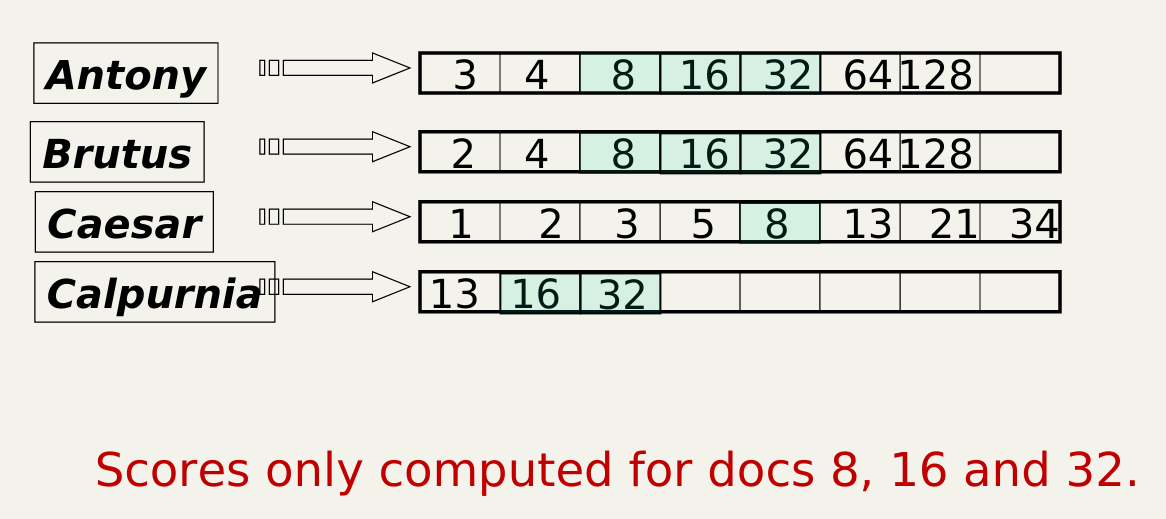
\includegraphics[width=0.8\textwidth]{Images/highIDF}
		 \caption{Top-k documents using high-IDF}
		 \label{img:highIDF}
	 \end{figure}

   \item We use \emph{Champion lists}, where we assign to each term, its
	 $m$ best documents, so if $|Q| = q$ terms we merge their preffered
         lists ($\leq mq$ answers) and we compute the cosine between $q$
	 and these docs, and choose the top.\newline
	 This approach need to pick $m > k$ to work well empirically.

   \item We use \emph{Fancy-hits} heuristic, where we assign docID by
	 decreasing PR weight, sort by docID $=$ order by decreasing 
	 PR weight, so we define $FH(t) = m$ docs for $t$ with 
	 highest $tf$-$idf$ weight and we define $IL(t)$ as the rest.

	 To search a $t-$term query we use a double approach:
	 \begin{enumerate}
	    \item consider $FH$ and we compute the score of all docs in their
		  $FH$, like champion lists and keep the top$-k$ docs.
	    \item consider then $IL$, so we scan $IL$s and check the common 
		  docs: compute the score, possibly insert them into 
		  the top$-k$ and stop when $m$ docs have been checked or
		  the $PR$ score becomes smaller than some threshold.
	 \end{enumerate}
         In figure \ref{img:fancy} it is possible to understand when we 
	 stop to consider elements in fancy-hits approach.

	 \begin{figure}
		 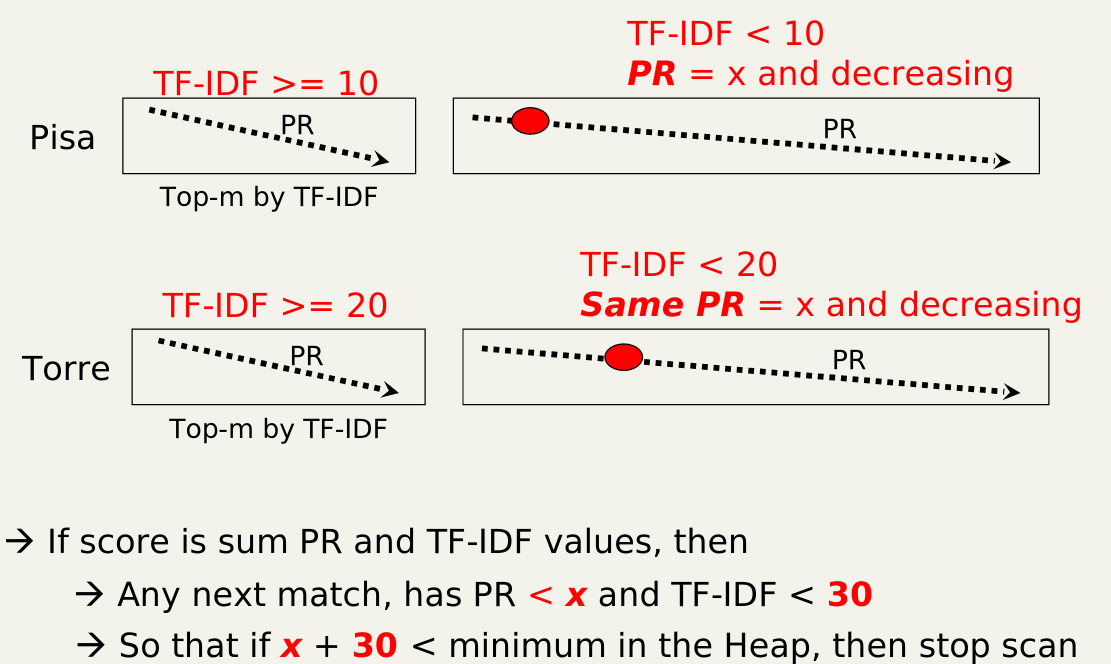
\includegraphics[width=0.8\textwidth]{Images/fancyHits}
		 \caption{Stop criteria for Fancy-hits approach}
		 \label{img:fancy}
	 \end{figure}
	 We assign to each document a query-independent quality score in
	 $[0, 1]$ to each document $d$ (denote this by $g(d)$ and thus
	 a quantity like the number of citation is scaled into $[0, 1]$.\newline
	 We can combine champion lists with $g(d)$ ordering, or maintain
	 for each term a champion list of the $r > k$ docs with highest 
	 $g(d) + tf-idf_{td}$; $g(d)$ may be the PageRank and seek top $k$
	 results from only the docs in these champion lists.

    \item The last but not least approach consist to clustering, where we 
	  pick $\sqrt N$ docs at random (call these leader) and for every
	  other doc we precompute nearest leader, so docs are attached
	  to a leader and each leader has $\sim N$ followers.

	  It process a query as follows:
	  \begin{enumerate}
	      \item Given query $Q$ find its nearest leader $L$.
	      \item Seek $K$ nearest docs from among $L$'s followers.
	  \end{enumerate}
	  We use a random sampling because it is fast and leaders 
	  reflect data distribution, anyway we will study now a general 
	  variant, which consist that each followe is attached to the 
	  nearest leader, but given now the query find for example $b=4$
	  nearest leaders and their followers.\newline
	  For them compute the scores and then take the top$-k$ ones
	  and that can recur on leader/follower construction.

\end{itemize}

\section{Exact top-$k$ documents}
In this section we will consider the problem that given a query $Q$
find the exact top $k$ docs for $Q$, using some ranking function $r$.

The simplest strategy consist to:
\begin{enumerate}
    \item Find all documents in the intersection.
    \item Compute score $r(d)$ for all these documents $d$.
    \item Sort results by score. 
    \item Return top $k$ results.
\end{enumerate}
The problem of this approach is that the score computation is a large fraction
of the CPU work on a queery and our goal is to cut CPU usage for scoring,
without compromising on the quality of results and the basic idea consist
to avoid scoring docs that won't make it into the top $k$.

A better approach consist to \emph{WAND} technique, a pruning method which
uses a max heap over the real document scores, and there is a proof that 
the docIDs in the heap at the end of the process are the exact top$-k$.

Basic idea of this approach come from the \emph{branch and bound}, so 
we maintain a running threshold score ($k$-th highest score computed so far),
we prune away all docs whose scores are guaranteed to be below the threshold
and in the end we compute exact scores for only the unpruned docs.

In WAND postings are ordered by docID, and we assume a special iterator on the 
postings that can go to the first docID $>$ X (using skip pointers or 
Elias-Fano's compressed lists) and this iterator moves only to the right,
to larger docIDs.

We assume also that $r(t, d)$ is the score of $t$ in $d$ and the score of the 
document $d$ is the sum of the scores of query terms; also for each query 
term $t$, there is some upper-bound $UB(t)$ such that, for all $d$
\[ r(t, d) \leq UB(t) \]
and these values are pre-computed and stored.

We keep inductively a threshold $\theta$ such that for every document $d$
within the top-$k$ it holds that $r(d) \geq \theta$; $\theta$ can be initialized
to $0$ and it is raised whenever the "worst" currently found top$-k$ has a 
score above the threshold.

In figure \ref{img:wand} it is possible to note the execution of WAND approach
and in test wand leads to a $90\%$ reduction in score computation (better
gains are on longer queries and gives us also safe ranking.

\begin{figure}
	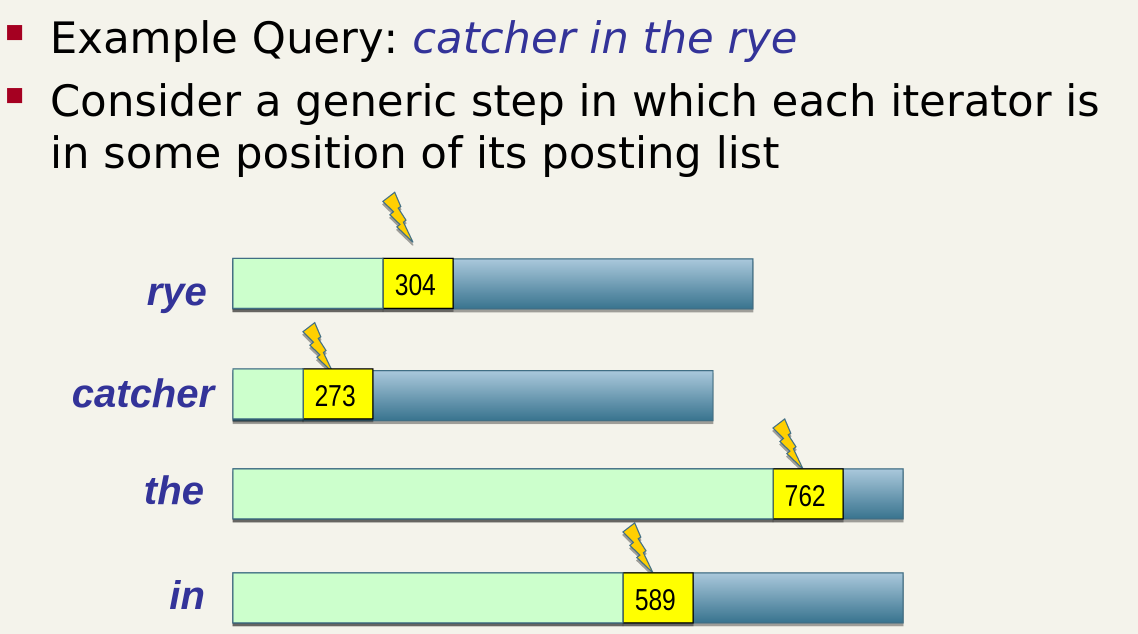
\includegraphics[width=0.4\textwidth]{Images/wand1}
	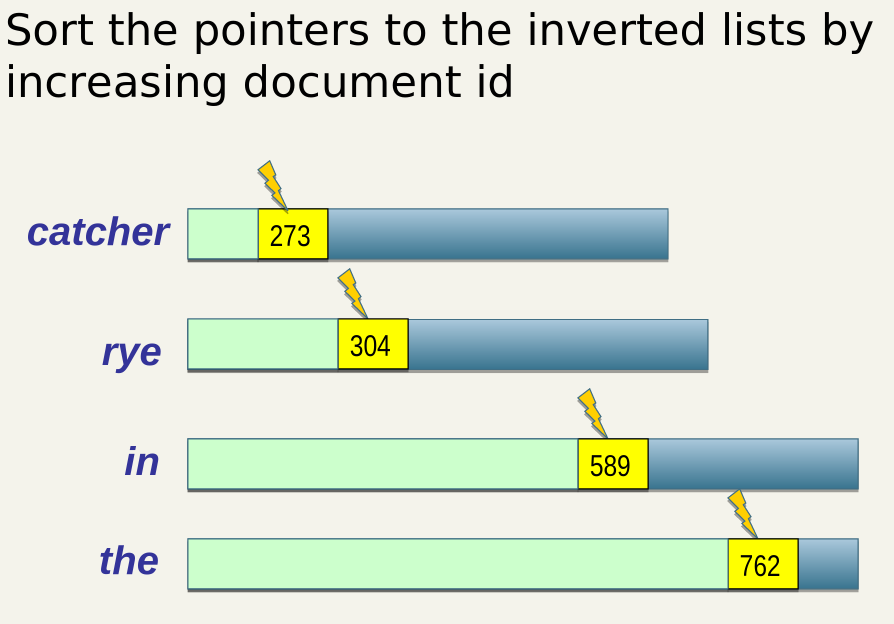
\includegraphics[width=0.4\textwidth]{Images/wand2}
	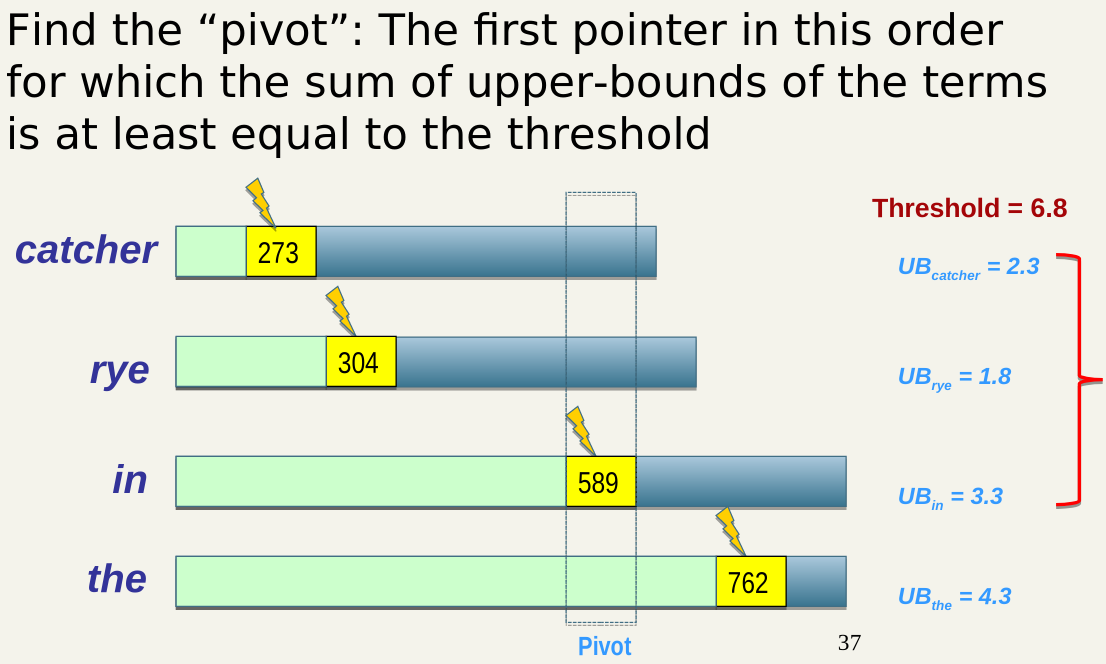
\includegraphics[width=0.4\textwidth]{Images/wand3}
	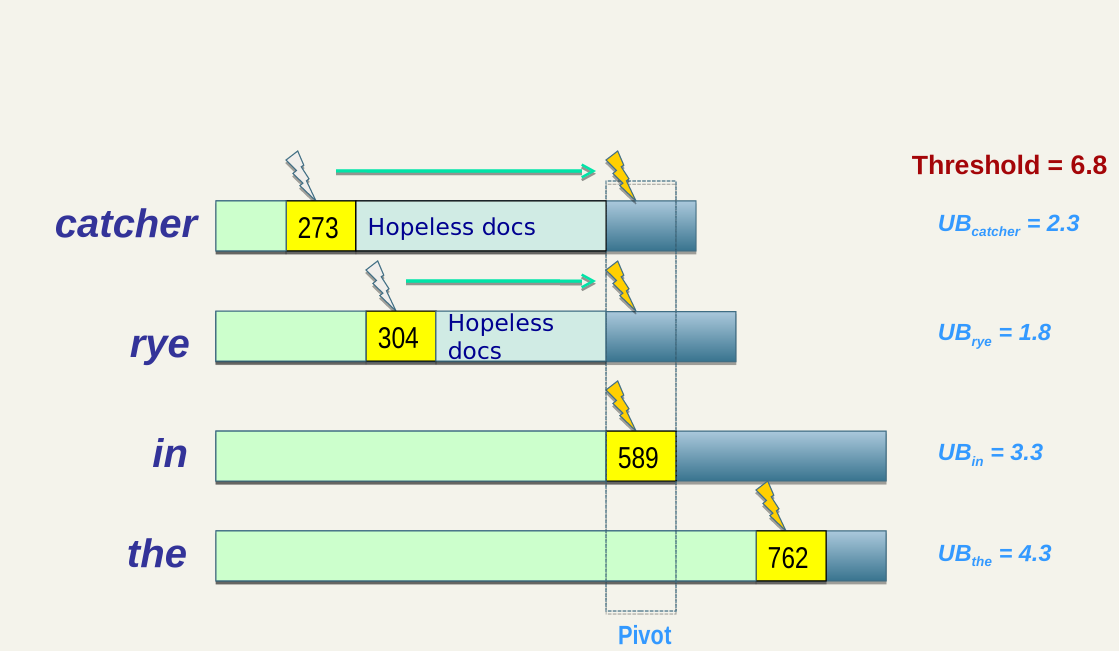
\includegraphics[width=0.4\textwidth]{Images/wand4}
	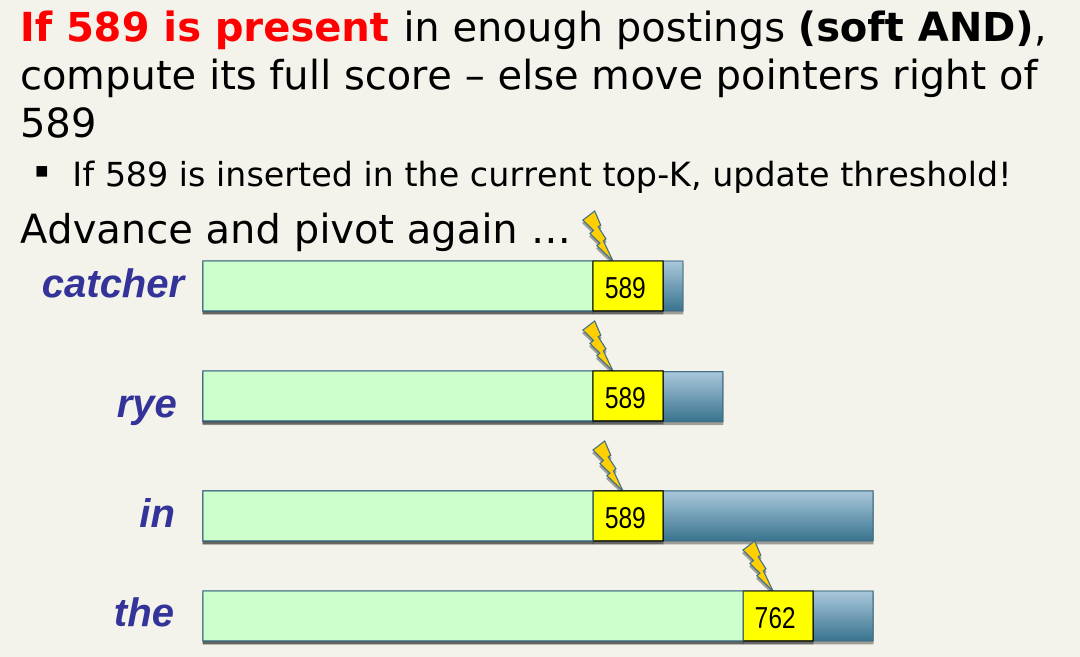
\includegraphics[width=0.4\textwidth]{Images/wand5}
	\caption{Execution of Wand algorithms steps}
	\label{img:wand}
\end{figure}

In wand $UB(t)$ was over the full list of $t$ and to improve this we add the 
following: partition the list into blocks and store for each block $b$ the 
maximum score $UB_b(t)$ among the docIDs stored into it, so we have 
the new algorithm \emph{block-max WAND}, that consist in $2-$levels check.

As in previous WAND we compute $p$, pivoting docIDs via threshold $\theta$
taken from the max-heap and let also $d$ be the pivoting docID in list($p$).

The new aspects executed in block-max variant is visible in figure 
\ref{img:blockWand}.

\begin{figure}
	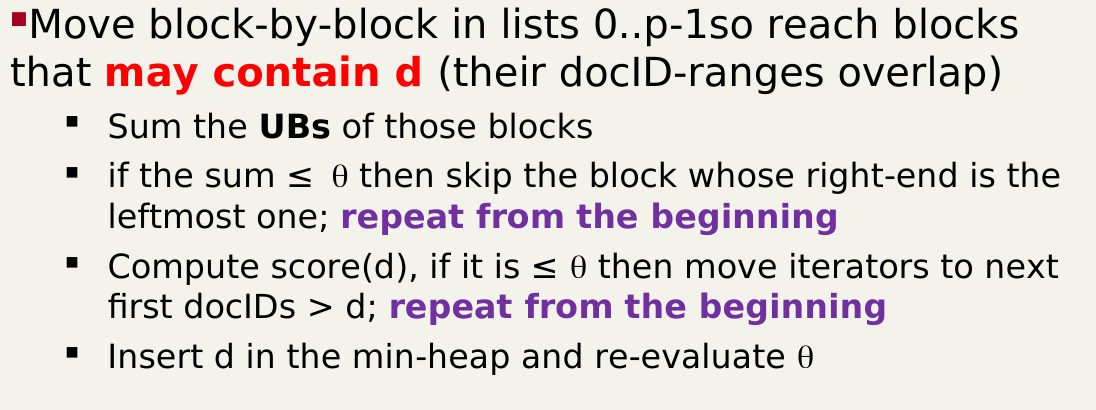
\includegraphics[width=0.7\textwidth]{Images/blockWand}
	\caption{Block-max Wand approach extension}
	\label{img:blockWand}
\end{figure}

\section{Relevance Feedback}
Relevance feedback consist that user give feedback on relevance of docs
in initial set of results, with an approach that consist on
\begin{itemize}
    \item User issues a (short, simple) query.
    \item The user marks some results as relevant or non-relevant.
    \item The system computes a better representation of the information
	  need based on feedback.
    \item Relevance feedback can go through one of more iterations.
\end{itemize}
A measure communly used is the \emph{Rocchio (SMART)} which is defined as
\[ q_m = \alpha q_0 + \beta \frac{1}{|D_r|} \sum _{d_j \in D_r} d_j -
         \gamma \frac{1}{|D_{nr}|} \sum _{d_j \in D_{nr}} d_j \]
where $D_r$ is the set of known relevant doc vectors, $D_{nr}$ is the 
set of known irrelevant doc vectors, $q_m$ is modified query vector
and $q_0$ is the original query vector.

With this formula new query moves toward relevant documents and away
from irrelevant documents, but the problem of this relevant approach 
consist that users are often reluctant to provide explicit feedback,
also it's often harder to understand why a particular document was retrieved
after applying relevance feedback and in the end there is no clear evidence
that relevance feedback is the "best use" of the user's time.

An improvement consist to \emph{Pseudo relevance feedback}, which
automates the "manual" part, so we retrieve a list of hits for the
user's query, assume that the top $k$ are relevant and do relevance feedback.

This pseudo approach works very well on average, but can go horribly wrong
for some queries and several iterations can cause query drift.

In relevance feedback, users give additional input (relevant/non-relevant)
on documents, which is used to reweight terms in the documents and 
in query expansion, users give additional input (good/bad search term)
on words or phrases; ways to augment the user query are manual thesaurus
(costly to generate using for example MedLine), global analysis (static)
done on all docs in collection using automatically derived thesaurus and 
refinements based on query-log mining and the last approach consist to
local analysis (dynamic), which consist to analysis of documents in result set.

\section{Quality of Search Engine}
In this section we will consider the quality of search engine, and provide
so measure functions to evaluate search engine but also all information
retrieval systems.

Some measures to evaluate can be how fast does it index, how fast does
it search, expressiveness of the query language and these criteria are
measurable but the key measure is the \emph{user happiness}, because
useless answers won't make a user happy, so we introduce two important 
measures: \emph{precision} and \emph{recall}.

In figure \ref{img:precisionRecall} is possible to note visually what 
mean these measure, but in words precision is the percentual
of docs retrieved that are relevant, instead recall is the 
percentual of docs relevant that are retrieved.

\begin{figure}
	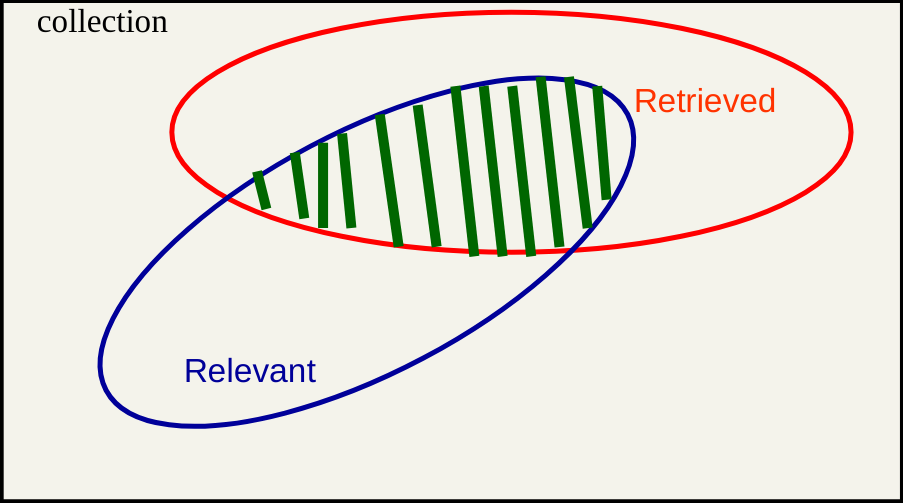
\includegraphics[width=0.8\textwidth]{Images/precisionRecall}
	\caption{Meaning of Precision and Recall}
	\label{img:precisionRecall}
\end{figure}

In figure \ref{img:relevantMatrix} is possible to note the table between
retrieved and relevant so from them can be derived the formula
of these criteria
\begin{align*}
	P & = \frac{TP}{TP + FP} \\
	R & = \frac{TP}{TP + FN} \\
\end{align*}
In the end in figure \ref{img:imagePrecision} is possible to note
the relation between precision and recall displayed by a plot.

\begin{figure}
	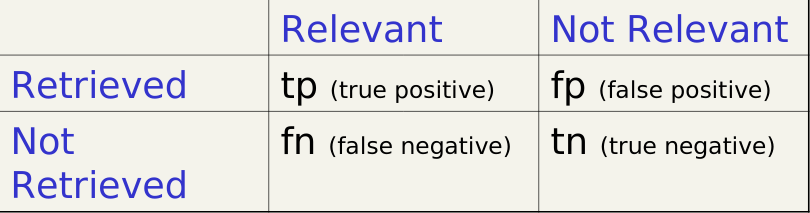
\includegraphics[width=0.8\textwidth]{Images/relevantMatrix}
	\caption{Relation between Relevant and Retrieved documents}
	\label{img:relevantMatrix}
\end{figure}
Last but not least measure used is the \emph{F measure}, that it is 
a combined measure (weighted harmonic mean) defined as 
\[ F = \frac{1}{\alpha \frac{1}{P} + (1 - \alpha) \frac{1}{R}} \]
People usually use balanced $F_1$ measure with $\alpha = 0.5$.

\begin{figure}
	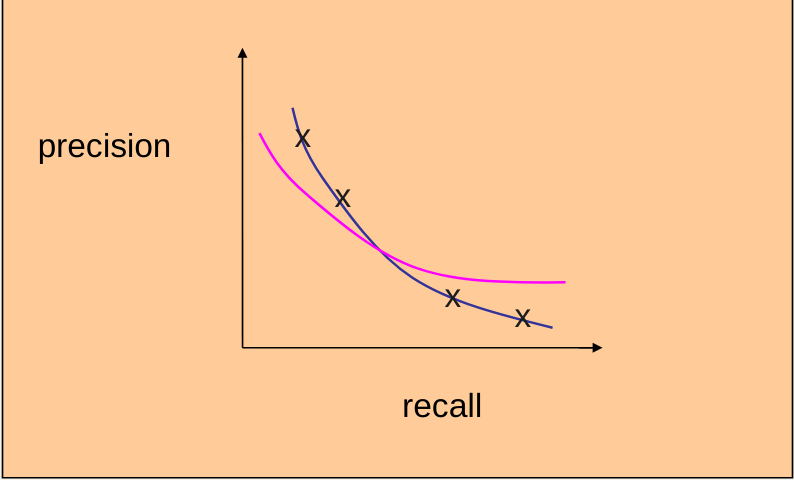
\includegraphics[width=0.7\textwidth]{Images/precisionCurve}
	\caption{Precision-Recall curve}
	\label{img:imagePrecision}
\end{figure}
